\documentclass[]{article}
\usepackage{lmodern}
\usepackage{amssymb,amsmath}
\usepackage{ifxetex,ifluatex}
\usepackage{fixltx2e} % provides \textsubscript
\ifnum 0\ifxetex 1\fi\ifluatex 1\fi=0 % if pdftex
  \usepackage[T1]{fontenc}
  \usepackage[utf8]{inputenc}
\else % if luatex or xelatex
  \ifxetex
    \usepackage{mathspec}
  \else
    \usepackage{fontspec}
  \fi
  \defaultfontfeatures{Ligatures=TeX,Scale=MatchLowercase}
\fi
% use upquote if available, for straight quotes in verbatim environments
\IfFileExists{upquote.sty}{\usepackage{upquote}}{}
% use microtype if available
\IfFileExists{microtype.sty}{%
\usepackage{microtype}
\UseMicrotypeSet[protrusion]{basicmath} % disable protrusion for tt fonts
}{}
\usepackage[margin=1in]{geometry}
\usepackage{hyperref}
\hypersetup{unicode=true,
            pdftitle={Zailtasunak adizkian. Non?},
            pdfauthor={Juan Abasolo},
            pdfkeywords={zailtasunak, euskara H2 berantiarra, adizkia, banaketa, explorazio (?!)
ikerketa},
            pdfborder={0 0 0},
            breaklinks=true}
\urlstyle{same}  % don't use monospace font for urls
\usepackage{longtable,booktabs}
\usepackage{graphicx,grffile}
\makeatletter
\def\maxwidth{\ifdim\Gin@nat@width>\linewidth\linewidth\else\Gin@nat@width\fi}
\def\maxheight{\ifdim\Gin@nat@height>\textheight\textheight\else\Gin@nat@height\fi}
\makeatother
% Scale images if necessary, so that they will not overflow the page
% margins by default, and it is still possible to overwrite the defaults
% using explicit options in \includegraphics[width, height, ...]{}
\setkeys{Gin}{width=\maxwidth,height=\maxheight,keepaspectratio}
\usepackage[normalem]{ulem}
% avoid problems with \sout in headers with hyperref:
\pdfstringdefDisableCommands{\renewcommand{\sout}{}}
\IfFileExists{parskip.sty}{%
\usepackage{parskip}
}{% else
\setlength{\parindent}{0pt}
\setlength{\parskip}{6pt plus 2pt minus 1pt}
}
\setlength{\emergencystretch}{3em}  % prevent overfull lines
\providecommand{\tightlist}{%
  \setlength{\itemsep}{0pt}\setlength{\parskip}{0pt}}
\setcounter{secnumdepth}{0}
% Redefines (sub)paragraphs to behave more like sections
\ifx\paragraph\undefined\else
\let\oldparagraph\paragraph
\renewcommand{\paragraph}[1]{\oldparagraph{#1}\mbox{}}
\fi
\ifx\subparagraph\undefined\else
\let\oldsubparagraph\subparagraph
\renewcommand{\subparagraph}[1]{\oldsubparagraph{#1}\mbox{}}
\fi

%%% Use protect on footnotes to avoid problems with footnotes in titles
\let\rmarkdownfootnote\footnote%
\def\footnote{\protect\rmarkdownfootnote}

%%% Change title format to be more compact
\usepackage{titling}

% Create subtitle command for use in maketitle
\newcommand{\subtitle}[1]{
  \posttitle{
    \begin{center}\large#1\end{center}
    }
}

\setlength{\droptitle}{-2em}
  \title{Zailtasunak adizkian. Non?}
  \pretitle{\vspace{\droptitle}\centering\huge}
  \posttitle{\par}
  \author{Juan Abasolo}
  \preauthor{\centering\large\emph}
  \postauthor{\par}
  \predate{\centering\large\emph}
  \postdate{\par}
  \date{2018-08-08 11:09:11}

\usepackage[basque]{babel}
\usepackage{apacite}
\bibliographystyle{apacite}

% ALDAKETAK

%Taulak eta irudijak atzekoz aurrera aldatu
\makeatletter 
\renewcommand{\fnum@figure}{\thefigure.~\figurename}
\renewcommand{\fnum@table}{\thetable.~\tablename}
\makeatother

\begin{document}
\maketitle
\begin{abstract}
Artikulu honetan aurkezten da euskara ikastun baten berbazko
ekoizpenaren analisi bat; fokua adizkiaren inguruan neurtutako
zailtasunetan kokatzen da, ea aditz nagusiak, adizki laguntzaileak ala
zeren inguruan multzokatzen diren erabaki nahirik. Horretarako
zailtasunen banaketen ondarrak \(\chi^2\) banaketarekin alderatu da.
Ikastun honen kasuan zailtasunak adizki trinko jokatu edo adizki
laguntzaileen inguruan multzokatzen direla aurkitu dugu.
\end{abstract}

\section{Sarrera}\label{sarrera}

Lan honetan erakusten da adizki jokatuaren elementuen sailkapen bat,
zeinetan adizki nagusi perifrastikoak elementu erraztzat antzematen den
eta adizki trinko zein laguntzaileek beste talde bat osatzen dutela
ematen duen, adizkiaren alderdi zaila.

Aurkezten ditugun datuak ikerketa handiagoan ulertu behar dira, euskara
ikastun batek ahozko ekoizpenean erakutsitako zailtasunaren analisian
(Abasolo, 2017), hain zuzen. Lan horretan eta beste batzuetan (Abasolo,
2015a, 2016) erakutsia da zailtasuntzat har litezkeen errore, fonazio
luzatu, errepikapen eta birformulazio zenbaitek antzerako portaera
erakusten dutela.

{[}HURRENGU AZTERTU ETA EGOKITU{]}: Hizkuntza-ekoizpena azaltzeko
Speaking liburuan (Levelt, 1989) aurkeztu zen ereduak H1eko ekoizpena
baino ez zuen hartu kontuan. De Bot-en ekarpenari (De Bot, 1992) heldu
zion Segalowitzek (Segalowitz, 2010); besteak beste, ekoizpen uneko
etorri etenak aztertzeko.

\begin{figure}

{\centering 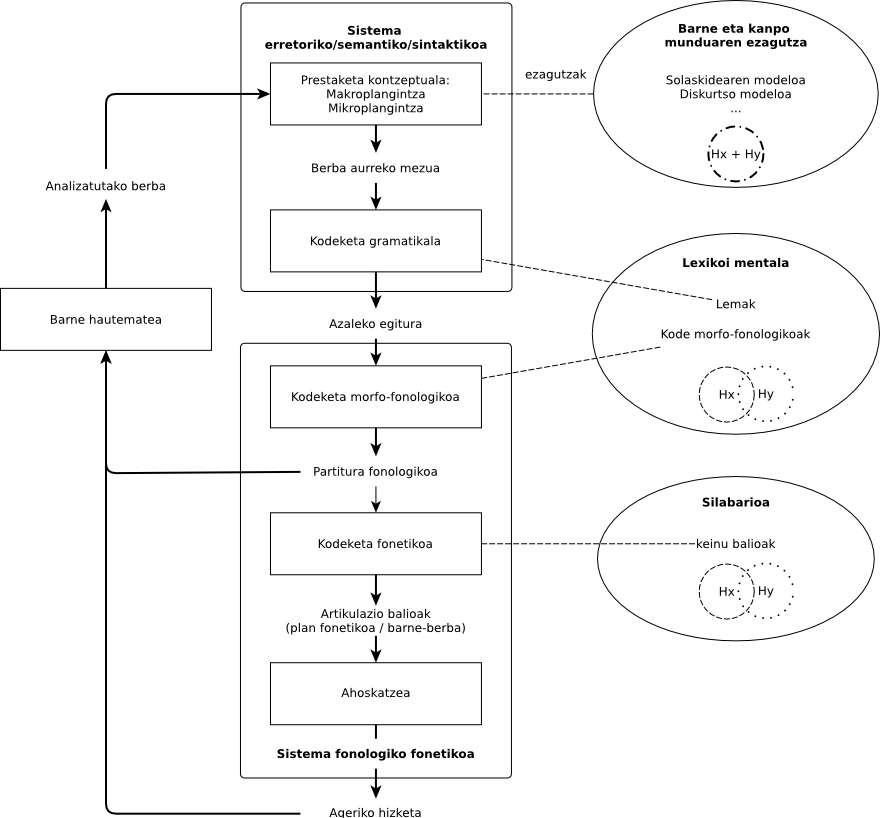
\includegraphics[width=0.8\linewidth]{./grafikoak/Levelten_eredua_Nik-garden} 

}

\caption{Levelten Hizketaren eredua H~2~ ere kontuan hartuta}\label{fig:levelt}
\end{figure}

Hizketaren prozesamendu horretan, Kormosek dioenez, bigarren hizkuntza
batean ari den ikastunak kodetze gramatikalik ez du eraikitzen, baizik
eta elementuen formaren arabera aukeratzen ditu Lexikoi Mentalean
(Kormos, 2006), irudian erdiko biribilean irudikatzen dena.

Hizketa ekoizte uneko ezaugarri dira zalantzak eta autozuzenketak,
H\textsubscript{1} zein H\textsubscript{2} izan. Errakuntzak denean
ematen badira ere, H\textsubscript{2}ko gaitasun baxuko ikasleena dela
ere esan ohi da. Ikerketa honetan darabilgun corpuseko datuetan
zalantza, autozuzenketa eta erroreak aditz jokatuaren inguruan kokatzen
dira.

\begin{figure}

{\centering 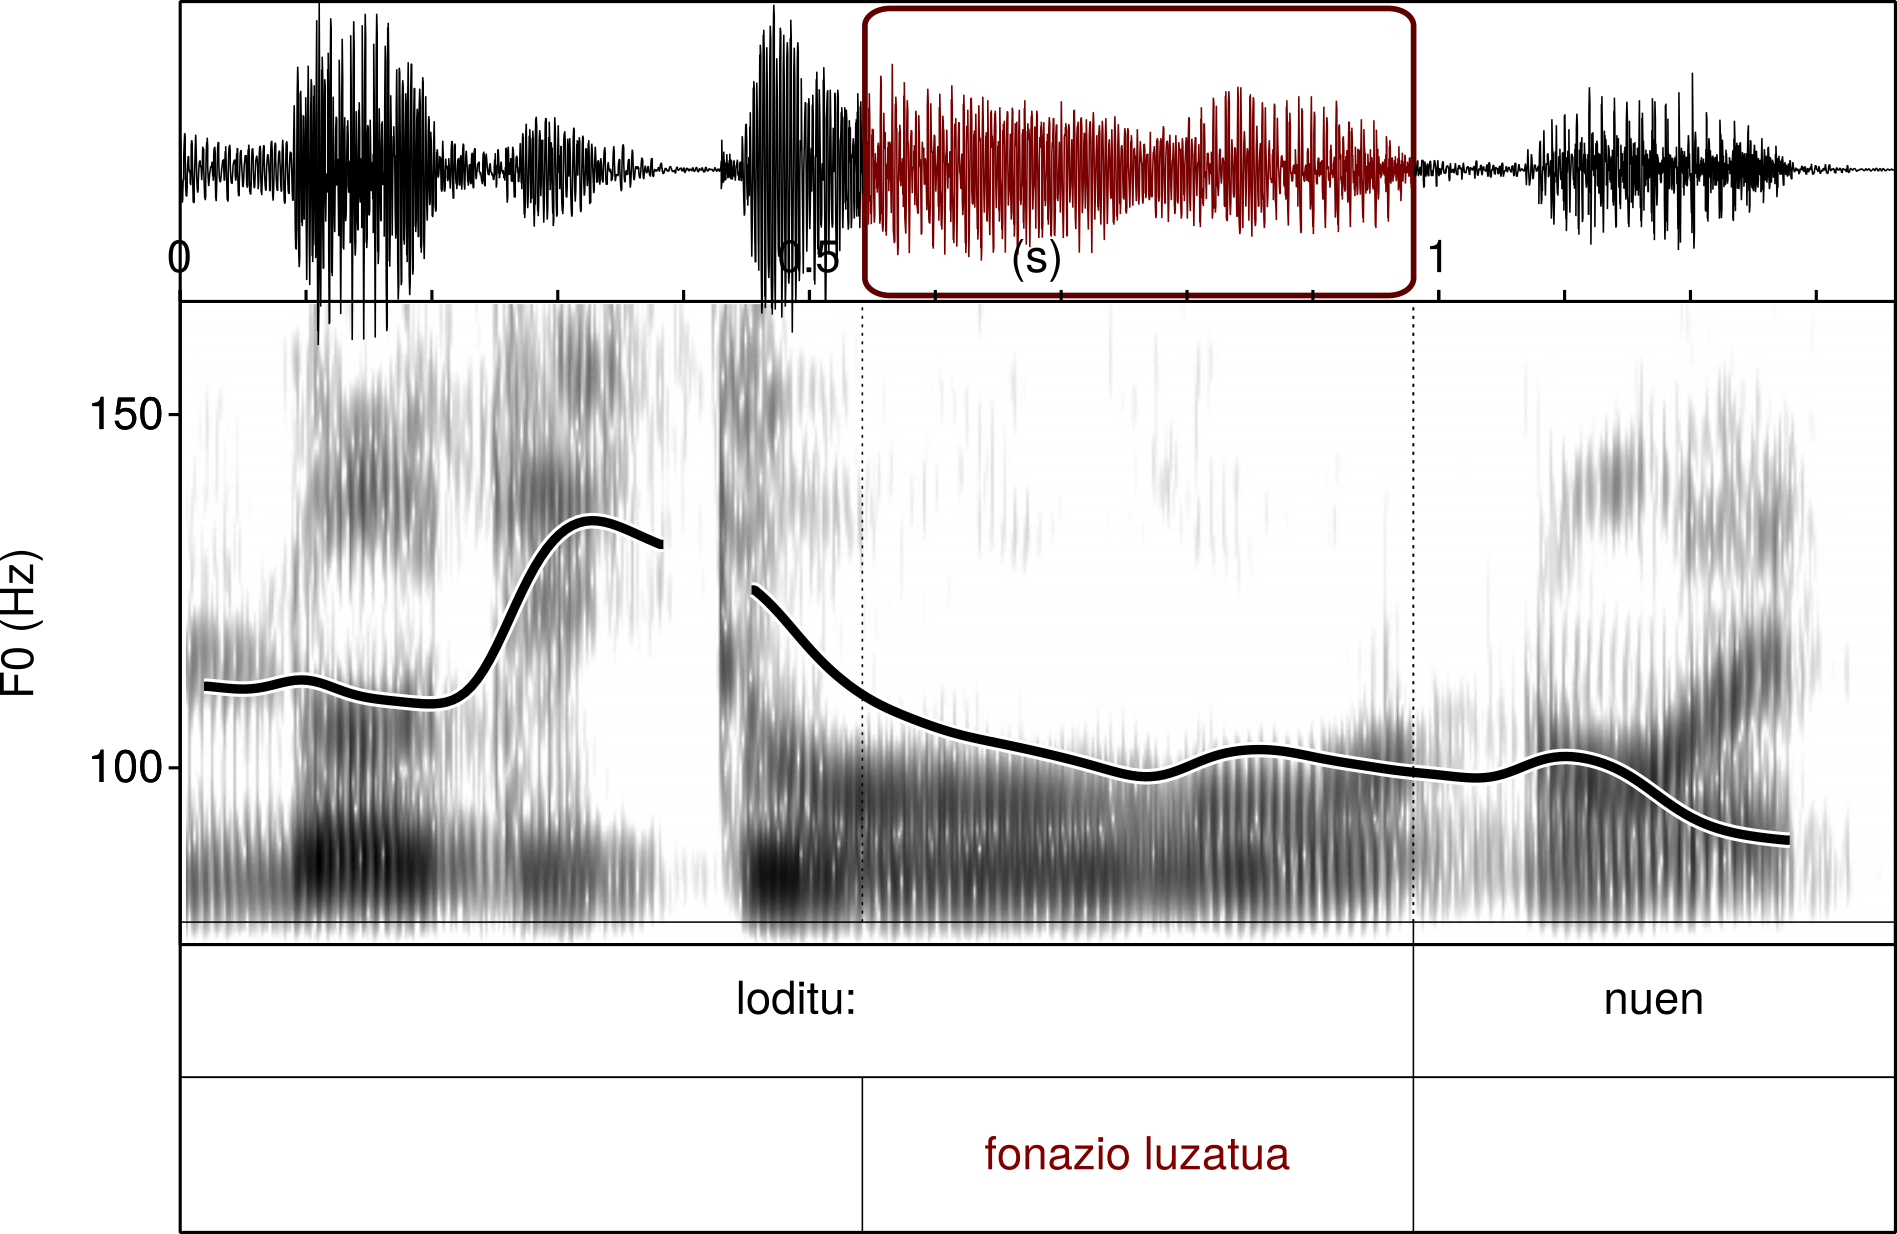
\includegraphics[width=0.8\linewidth]{./grafikoak/luz1} 

}

\caption{Fonazio luzatuaren irudi bat PRAAT erabilita}\label{fig:unnamed-chunk-1}
\end{figure}

Zailtasun adierazletzat hartzen da zalantza adierazleetatik gramatika
erroreetaraino dirauen continuuma, (Gaëtanelle \& De Cock, 2011) lanetan
iradoki eta (Abasolo, 2017) lanean sailkatu den moduan:

\paragraph{Zailtasunen continuuma}\label{zailtasunen-continuuma}

\begin{itemize}
\tightlist
\item
  Ahoskatu gabeak

  \begin{itemize}
  \tightlist
  \item
    Zalantza isilak
  \end{itemize}
\item
  Ahoskatuak

  \begin{itemize}
  \tightlist
  \item
    Zalantzak

    \begin{itemize}
    \tightlist
    \item
      Fonazio luzatuak
    \item
      Silabaz silabako ahoskera
    \item
      Errepikapenak
    \end{itemize}
  \item
    Erroreak

    \begin{itemize}
    \tightlist
    \item
      Hautemandakoak

      \begin{itemize}
      \tightlist
      \item
        Zuzendutakoak\\
        Errepikapenak\\
        Berba zatiak\\
        Birformulazioak\\
      \item
        Zuzendu gabekoak
      \end{itemize}
    \item
      Hauteman gabekoak
    \end{itemize}
  \end{itemize}
\end{itemize}

Irudian ikusten den zalantza adierazlea fonazio luzatua da, aurreko
zerrendako hasierako elementuetako bat; zalantza hori adizki jokatuan
kokatzen da, aditz nagusiaren alderdian, hain zuzen. Adizki
laguntzailearen aurre-aurrean.

Euskarazko aditz jokatuak zenbait ikertzaile liluratu du, ez dago
besterik ingelesezko\footnote{\url{https://en.wikipedia.org/wiki/Basque_verbs}}
edo gaztelaniazko\footnote{\url{https://es.wikipedia.org/wiki/Verbo_vasco}}
wikipediako artikuluen hasierak irakurtzea baino. Argiro azaltzen du
MorenoCabrerak falazia batez ari garela hizkuntzaren konplexutasun
gramatikalaz ari garenean {[}@ MorenoCabrera\_XXXX{]}. Oposizioak
markatzen baitu aldearen tamaina, oposizioa egoteak ala ez egoteak
(Newmeyer \& Preston, 2014), eta ez forma kopuruak.

Beste alde batetik, euskarazko adizki jokatuak hainbat informazio
barnebil ditzake, H\textsubscript{2}an trebatzen ari denean zailtasun
eragile izan daitezkeena.

\begin{enumerate}
\def\labelenumi{(\arabic{enumi})}
\item
  Etor zitezkeen
\item
  Badago
\end{enumerate}

Goiko adibideetako kasuetan ikus dezakegu
\protect\hyperlink{etorzitezkeen}{lehenengo kasuan} adizki perifrastiko
horretan adizki nagusiak baduela informa.zio semantikoa. Bigarrenak,
adizki laguntzaileak, berriz, ia erabat erantsia du informazio
semantikoa aditz nagusi gabe. Baina, era berean, informazio asko kodetu
edo aukeratu behar da, baldin eta ikastunak horixe argi adierazi behar
badu euskaraz. \protect\hyperlink{badago}{Bigarren adibidean}, berriz,
batean ikusten dira adizkiaren informazio semantikoa, \emph{egotea}, eta
horri dagozkion modu, pertsona eta zenbaki informazioa.

EGA azterketako idatziaren analisian Pello Esnalek oso errakuntza gutxi
aurkitu zituen 1988ko bere tesinan eta honela azaltzen zuen:

\begin{quote}
aditzaren arloa dugu euskal hizkuntz formen artean egituratuenetarikoa

---\emph{{[}@ Pello Esnal (1988){]}}
\end{quote}

Idatzitakoaren analisiak, zailtasunen continuumean, errakuntzen berri
baino ezin liteke eman; horra ahozko jardunaren analisiak duen azalpen
ahalmen handiagoa.

\subsubsection{Corpusa}\label{corpusa}

Datuak urtebetean zehar batu ziren, 2014-2015 ikasturtean zehar.
Horretarako ikastunari grabatu zitzaizkion zenbait ahozko ariketa,
aurrez prestatutako mologoa egitean dautzana.

Ikerketa honetarako propio garatutako transkribatze eta etiketatze
sistema erabili zen (Abasolo, 2015b). Kodeketa horretan grafema
bakarreko edo biko etiketak erabili ziren zailtasun adierazle bakoitza
identifikatzeko, baita zenbait ezaugarri morfosintaktiko nabarmentzeko
ere. Bigarren pausu batean, etiketen multzokatze motak nola banatzen
diren ikusteko bidea ematen du kodetutako testuaren azterketak.

\begin{longtable}[]{@{}llll@{}}
\caption{Testu eta etiketen adibidea}\tabularnewline
\toprule
esaldia: & @æ \emph{jakiteko betebeharrak} & \$ \emph{betetze:n} & ¡
\emph{duten} *2\tabularnewline
\midrule
\endfirsthead
\toprule
esaldia: & @æ \emph{jakiteko betebeharrak} & \$ \emph{betetze:n} & ¡
\emph{duten} *2\tabularnewline
\midrule
\endhead
etiketak & & luzatua0 & luzatua1\tabularnewline
& & & errorea (eza)\tabularnewline
& aditz argmentua ABS & aditz nagusia & adizki
laguntzailea\tabularnewline
\bottomrule
\end{longtable}

Corpusaren ezaugarri kuantitatiboak aurkezten dira hurrengo taulan

\begin{longtable}[]{@{}ll@{}}
\caption{Aztertutako corpusaren ezaugarriak}\tabularnewline
\toprule
\begin{minipage}[b]{0.47\columnwidth}\raggedright\strut
3057 berba\strut
\end{minipage} & \begin{minipage}[b]{0.47\columnwidth}\raggedright\strut
1325 zailtasun\strut
\end{minipage}\tabularnewline
\midrule
\endfirsthead
\toprule
\begin{minipage}[b]{0.47\columnwidth}\raggedright\strut
3057 berba\strut
\end{minipage} & \begin{minipage}[b]{0.47\columnwidth}\raggedright\strut
1325 zailtasun\strut
\end{minipage}\tabularnewline
\midrule
\endhead
\begin{minipage}[t]{0.47\columnwidth}\raggedright\strut
14 monologo3057 berba 467 adizki * 304 adizki nagusi perifrastiko / 278
adizki laguntzaile * 189 adizki trinko407 aditz argumentu 64 Ezezko
partikula\strut
\end{minipage} & \begin{minipage}[t]{0.47\columnwidth}\raggedright\strut
564 fonazio luzatu38 berba silabatze markatuaz275 osatu gabeko berba66
errepikapen144 birformulazio\sout{238 errore}\strut
\end{minipage}\tabularnewline
\bottomrule
\end{longtable}

Datuen ezaugarri morfosintaktikoen arabera aztertu dira zailtasunen
banaketak, gehienetan, \(\chi^2\)arenarekin alderatuta. Horrela, aurkitu
ahal izan dugu zenbait ezaugarrik badutela aditzen inguruko banaketa
bereizia.

\begin{longtable}[]{@{}lcccc@{}}
\caption{Zailtasunen eta ezaugarri morfosintaktikoen banaketaren
adierazgarritasun mailak, \(\chi^2\) banaketaren
arabera.}\tabularnewline
\toprule
Zailtasunen menpeko banaketak (\(\chi^2\)) & \textbf{\emph{ez}} &
\textbf{aditz nagusia} & \textbf{trinkoa} &
\textbf{laguntzailea}\tabularnewline
\midrule
\endfirsthead
\toprule
Zailtasunen menpeko banaketak (\(\chi^2\)) & \textbf{\emph{ez}} &
\textbf{aditz nagusia} & \textbf{trinkoa} &
\textbf{laguntzailea}\tabularnewline
\midrule
\endhead
Fonazio luzatua & ** & *** & *** & ***\tabularnewline
Fonazio luzatua aurrekoan & & & *** & ***\tabularnewline
Fonazio luzatua azkenaurrekoan & & & & *\tabularnewline
Berba zatiak ahozkatu dira aurretik & ** & & *** & *\tabularnewline
Aurrekoaren errepikapena & *** & *** & ** & ***\tabularnewline
Errepikapena hasi eta geroko lehenengo berba da & & & * &
**\tabularnewline
Birformulazioa bertan hasten da & ** & & &\tabularnewline
Birformulazioa hasi eta geroko lehenengo berba da & & & ** &
***\tabularnewline
Zerbait falta du & & & & ***\tabularnewline
\bottomrule
\end{longtable}

Aurreko taulan ikusten denez, corpus honetan adizki nagusiaren zein
adizki laguntzaileen inguruan agertzen dira multzokatuta zailtasun
adierazleak. Corpus horretako datuen beste analisi bat proposatuko dugu
lan honetan.

\section{Hipotesiak}\label{hipotesiak}

Gure hipotesi nagusia da aditz nagusiaren inguruan aurkitu diren
zailtasunak, ez dagozkiola Aditz Nagusiari berari, baizik eta Adizki
Laguntzaileei. Eta hori hizketaren ekoizpenaren ezaugarri inkrementalak
azal lezake.

H\textsubscript{1}: Zalantza adierazleen multzokatzeak adizki
nagusietatik independenteak izango dira ezezko esaldietan.

H\textsubscript{2}: Bat datoz zalantza adierazleen banaketak adizki
laguntzaile zein adizki trinkoen kasuetan.

H\textsubscript{3}: Aditz nagusien aspektuetatik independentea da
zalantza adierazleen banaketa

\section{Metodologia}\label{metodologia}

Zailtasunen agerrera euskarazko adizkien ezaugarriren batek ala zerk
egiten duen zuzenean ezin aztertu daiteke corpusaren araketa hutsez,
bai, ordea, hobeto ezagutu horien elkarreraginak. Horixe aztertzea
helburu, hurrengo lerroetan aurkezten dugun lanerako ikusizko
azterketa-teknikak erabili ditugu, \emph{Visualizing Categorical Data}
(VCD), baneketen ezaugarrien ulerkuntzan sakontzeko (Friendly, 1994).R
estatistika lengoairako garatutako teknikak erabili ditugu (Meyer,
Zeileis, \& Hornik, 2006).

VCD teknikak tamainak erabiltzen ditu behatutako banaketa irudikatzeko,
koloreak konparaketa adierazgarriak erakusteko eta tonalitateak aldearen
indarra irudikatzeko.

Datuen banaketa mosaiko-grafiko batez irudikatzen du proportzioen berri
hartzeko. Alderaketa kolorez irudikatzen du, \(\chi^2\) egiten da
alderaketa gure kasuan, kolore gorriz erakusten ditu banaketa idealean
litzatekeena baino maiztasun gutxiago duten kategoriak eta kolore
urdinez alderatutakoaren gainetiko maiztasuna duten kategoriak.
Adierazgarritasunik erakusten ez duten multzokatzeetan grisa erabili
dugu lan honetan. Koloreon intentsitatea erabiltzen da aldea handiagoa
ala txikiagoa den erakusteko.

Aukera-arrazoia erabiltzeko joera dago 2x2 dimentsioetako alderaketak
egiteko, guk, lan honetarako horren erabilera baino \(\chi^2\)rena
lehenesten dugu arrazoi bigatik. Batetik, aukera-arrazoien indargunea
banaketaren aurretiko ezagutzan oinarritzen delako eta corpuseko datuak
ausaz hala hartuak izan direlako. Beste alderdi batetik, aurrez egindako
alderaketekin koherentzia gordetzeko, 2x2 taulok beste batzuen
erredukzioa direlako.

\subsubsection{Zalantza adierazleak eta adizki nagusiak independenteak
dira ezezko
esaldietan}\label{zalantza-adierazleak-eta-adizki-nagusiak-independenteak-dira-ezezko-esaldietan}

Alderaketa hau egiteko, fonazioak luzatzeko uneak eta berben balio
sintaktikoa alderatzen ditugu, zehazki ea adizki nagusia ala beste
zerbait diren. Kasu honetan alderatu behar ditugu elementuak
konfigurazio bitan: baiezko eta ezezko esaldietan.

\begin{figure}
\centering
\includegraphics{180808_artikulurantza_files/figure-latex/baietzNGvLZ0-1.pdf}
\caption{Fonazio luzatuak eta aditz nagusien banaketa baiezko
esaldietan}
\end{figure}

Irudian ikusten da, aditz nagusian fonazioa luzatzeko joera handia dela
aditz nagusietan baiezko esaldietan. Izan ere, konfigurazio horretan
etiketatutako fonazio luzatuen herenak aditz nagusian neurtu dira.
Kolore gorri argiak adierazten du fonazio luzatuak aukera baxuagoa duela
agertzeko aditz nagusia ez diren elementuetan. Hor irudikatuta dagoen
banaketak \(\chi^2\)(1, N=2157) = 33.138, p = 0 balioa du.

\begin{figure}
\centering
\includegraphics{180808_artikulurantza_files/figure-latex/ezetzNGvLZ0-1.pdf}
\caption{Fonazio luzatuak eta aditz nagusien banaketa ezezko esaldietan}
\end{figure}

Ezeko esaldietan, berriz, ez da antzematen ezelako joerarik irudian eta
alderik balego ere, adierazgarritasunik ez da ikusi \(\chi^2\)
banaketarekiko aldean honako balioa hartuta: \(\chi^2\)(1, N=413) = 0, p
= 1

\subsubsection{Zalantza adierazleen banaketak adizki laguntzaile eta
trinkoen
kasuetan}\label{zalantza-adierazleen-banaketak-adizki-laguntzaile-eta-trinkoen-kasuetan}

\begin{figure}
\centering
\includegraphics{180808_artikulurantza_files/figure-latex/laguntzaile-1.pdf}
\caption{Fonazio luzatua aurrekoan eta aditz trinkoak}
\end{figure}

\(\chi^2\)(1, N=2615) = 14.399, p = 1.5\times 10\^{}\{-4\}

\begin{figure}
\centering
\includegraphics{180808_artikulurantza_files/figure-latex/trinko-1.pdf}
\caption{Fonazio luzatua aurrekoan eta aditz laguntzailea}
\end{figure}

\(\chi^2\)(1, N=2615) = 13.805, p = 2\times 10\^{}\{-4\}

\subsubsection{Aditz nagusiaren aspektua eta fonazio
luzatua}\label{aditz-nagusiaren-aspektua-eta-fonazio-luzatua}

\begin{figure}
\centering
\includegraphics{180808_artikulurantza_files/figure-latex/adnagaspek-1.pdf}
\caption{Fonazio luzatua aditz nagusietan, aspektuen arabera}
\end{figure}

\(\chi^2\)(3, N=303) = 1.839, p = 0.60649

\section{Ondorioz}\label{ondorioz}

\begin{quote}
Aditz nagusiaren kokapena aditz laguntzaileak baldintzatzen duenez, hor
agertzen dira zalantza adierazle gehien adizki laguntzaileak edo
trinkoak baldintzatuta, eta ez aditz nagusiak berak edo aditz nagusia
ahoskatzeko egin beharreko gramatika kodeketa.
\end{quote}

\begin{quote}
Zalantza ahoskatzean, eragilea prozesatzen ari dela suposatu behar da,
emaitzen argitara. Antzeman ote daitezke, zalantzen kokapenaren arabera,
zein diren horien eragileak? Beste hiztun batzuen ahozko jardunean ere
aurkituko ditugu eaugarriok?
\end{quote}

\section*{Erreferentziak}\label{erreferentziak}
\addcontentsline{toc}{section}{Erreferentziak}

\hypertarget{refs}{}
\hypertarget{ref-abasolo_adizki_2015}{}
Abasolo, J. (2015a). Adizki jokatuen sailkapen hirukoitza: Zailtasunak,
etenak eta erroreak. In \emph{Nuevos retos en la investigación en
Psicodidáctica - Psikodidaktikako ikerkuntzaren erronka berriak} (6--20.
pp. ). Leioa: Argitarapen Zerbitzua, UPV/EHU.

\hypertarget{ref-abasolo_transkribatze_2015}{}
Abasolo, J. (2015b). Transkribatze arauak eta transkripzio helburuak. In
\emph{Investigar en psicodidáctica: Una realidad en auge -
Psikodidaktikako ikerketa gorabidean} (316--325. pp. ). Leioa:
Argitarapen Zerbitzua, UPV/EHU.

\hypertarget{ref-abasolo_desjariakortasuna_2016}{}
Abasolo, J. (2016). Desjariakortasuna eta gramatika errorea adizki
jokatuan B2-C1 ibilbidean: Kasu baten analisia. In \emph{XXIII Jornádas
de Invigación en psicodidáctica - XIII Psikodidaktikako ikerkuntza
jardunaldiak} (345--358. pp. ). Leioa: Argitarapen Zerbitzua, UPV/EHU.

\hypertarget{ref-abasolo_zailtasunak_2017}{}
Abasolo, J. (2017). \emph{Zailtasunak aditz jokatuaren inguruan B2-C1
ibilbidean} (Doktorego-tesia). UPV/EHU, Leioa. Berreskuratua editor \&
translator \url{https://addi.ehu.es/handle/10810/25306}-(e)tik

\hypertarget{ref-de_bot_bilingual_1992}{}
De Bot, K. (1992). A bilingual production model: Levelt's 'Speaking'
model adapted. \emph{Applied Linguistics}, \emph{13}(1), 1--24.

\hypertarget{ref-friendly_mosaic_1994}{}
Friendly, M. (1994). Mosaic Displays for Multi-Way Contingency Tables.
\emph{Journal of the American Statistical Association}, \emph{89}(425),
190.

\hypertarget{ref-gaetanelle_errors_2011}{}
Gaëtanelle, G., \& De Cock, S. (2011). Errors and disfluencies in spoken
corpora: Setting the scene. \emph{International Journal of Corpus
Linguistics}, \emph{16}(2), 141--172.

\hypertarget{ref-kormos_speech_2006}{}
Kormos, J. (2006). \emph{Speech Production and Second Language
Acquisition}. London: Lawrence Erlbaum Associates.

\hypertarget{ref-levelt_speaking:_1989}{}
Levelt, W. J. M. (1989). \emph{Speaking: From intention to
articulation}. Cambridge: The MIT Press.

\hypertarget{ref-meyer_strucplot_2006}{}
Meyer, D., Zeileis, A., \& Hornik, K. (2006). The Strucplot Framework:
Visualizing Multi-way Contingency Tables with vcd. \emph{Journal of
Statistical Software}, \emph{17}(3).

\hypertarget{ref-newmeyer_measuring_2014}{}
Newmeyer, F. J., \& Preston, L. B. (2014). \emph{Measuring Grammatical
Complexity}. Oxford University Press.

\hypertarget{ref-segalowitz_cognitive_2010}{}
Segalowitz, N. (2010). \emph{Cognitive Bases of Second Language
Fluency}. New York: Routledge.


\end{document}
